 %!TEX root = ./template-skripsi.tex
%-------------------------------------------------------------------------------
%                            BAB II
%               KAJIAN TEORI
%-------------------------------------------------------------------------------

\chapter{KAJIAN PUSTAKA} 

\section{\emph{Border Following}}

Salah satu teknik yang sering dipakai dalam pengolahan citra 
adalah \textit{Border Following}, terutama citra biner. 
\textit{Border following} telah diteliti oleh beberapa orang 
karena taknik ini memiliki pengaplikasian yang cukup luas, 
seperti pengenalan objek, analisis citra, deteksi objek, dan 
kompresi data citra (\cite{Suzuki})

Dalam penelitian yang dibuat oleh Suzuki, ia menawarkan 
dua algoritma \textit{border following} yang sampai saat ini 
masih digunakan oleh \textit{library} pengolahan citra yang 
umum diketahui yaitu \textbf{OpenCV}. Algoritma ini merupakan 
salah satu algoritma yang mengenalkan pendefinisian hubungan 
hierarki antar tepi (\textit{border}). Tidak hanya itu, 
algoritma ini juga membedakan tepi lubang (\textit{hole}) 
dan tepi luar (\textit{outer border}) di sebuah objek. 
Suzuki memberikan definisi pada algoritma ini, yaitu:
\begin{itemize}
	\item \textbf{Definisi 1 (\textit{border point})}.
	Sebuah piksel bernilai 1 yang dikelilingi oleh piksel
	bernilai 0 dapat disebut sebagai \textit{border point}.

	\item \textbf{Definisi 2 (komponen yang mengelilingi
	komponen lain.)}. Dari gambar 
	(\ref{gambar:Keliling_antar_komponen}) dapat dikatakan 
	bahwa komponen $S_2$ mengelilingi komponen $S_4$

	\item \textbf{Definisi 3(\textit{outer border} dan \textit{hole border})}. 
	Sebuah rangkaian \textit{border point} antar komponen yang 
	mempunyai nilai piksel 1 (objek) dengan komponen yang 
	mempunyai nilai piksel 0 (latar belakang)

	\item \textbf{Definisi 4(\textit{parent border})}. 
	Berdasarkan gambar (\ref{gambar:Keliling_antar_komponen}) 
	dapat dikatakan bahwa tepi $B_2$ adalah 
	\textit{parent border} dari tepi $B_3$

	\item \textbf{Definisi 5(tepian yang mengelilingi tepian 
	lain)}. Dari gambar (\ref{gambar:Keliling_antar_komponen}) 
	dapat dikatakan bahwa tepi $B_2$ mengelilingi tepi $B_3$.
\end{itemize}

\begin{figure}[H]
	\centering
	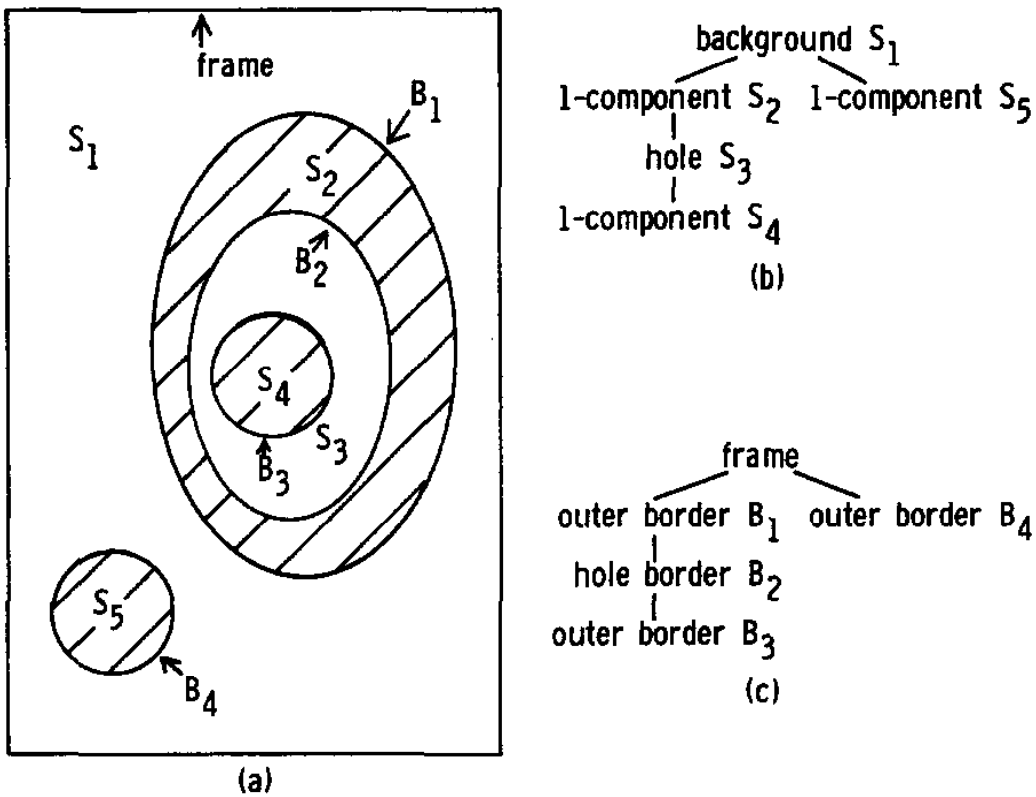
\includegraphics[keepaspectratio, width=10cm]{gambar/BorderFollowingPustaka/pic1.png}
	\caption{\textit{surroundness} antar komponen yang terhubung (b) 
	dan antar tepi(\textit{borders}) (c).}
	\label{gambar:Keliling_antar_komponen}
\end{figure}

Diasumsikan citra yang dimasukan algoritma ini 
berupa citra biner. Piksel dengan nilai 0 dan 1 
disebut sebagai 0-piksel dan 1-piksel. Nilai sebuah 
piksel dalam koordinat ($i,j$) yang masing-masing 
melambangkan baris dan kolom sebuah citra digital 
didefinisikan sebagai $f_{i,j}$. Baris paling pinggir
yang berada di atas, kanan, bawah, dan kiri adalah 
\textit{frame}(bingkai) dari citra tersebut. Dalam hal
ini, setiap tepi baru yang ditemukan akan diberi angka 
unik dan disebut sebagai \textbf{NBD}. Asumsikan NBD dari
\textit{frame} adalah 1, sementara tepi lain diberi angka 
NBD secara berurutan. Nilai NBD dari \textit{parent} 
setiap tepi di dalam variabel \textbf{LNBD} kemudian 
disimpan. Berikut merupakan langkah-langkah 
algoritma pertama \textit{border following}:

Dimulai dengan pemindaian piksel citra dari kiri ke kanan
hingga \textit{scanner} menemukan piksel objek 
($f_{i,j} \neq 0$). Dilanjutkan dengan menentukan 
apakah piksel tersebut merupakan tepi luar atau tepi 
lubang. Untuk setiap baris baru yang dipindai, 
kembalikan nilai LNBD ke 1.

\begin{enumerate}
	\item Langkah 1
	\begin{enumerate}[(a)]
		\item jika $f_{i,j} = 1$ dan $f_{i,j-1} = 0$, 
		maka piksel ($i,j$) adalah \textit{starting 
		point} dari operasi \textit{border following} 
		untuk tepi luar(\textit{outer border}). 
		inkremen NBD dan set ($i_2, j_2$) $\gets$ ($i, j-1$).
		\item jika $f_{i,j} \geq 1$ dan $f_{i,j+1} = 0$, 
		maka piksel ($i,j$) adalah \textit{starting 
		point} dari operasi \textit{border following} 
		untuk tepi lubang(\textit{hole border}). 
		inkremen NBD, set ($i_2, j_2$) $\gets$ ($i, j+1$), 
		dan LNBD $\gets f_{i,j}$ jika $f_{i,j} > 1$
		\item jika kedua kondisi tidak terpenuhi, maka
		lanjut ke langkah 4.
		\begin{figure}[H]
			\centering
			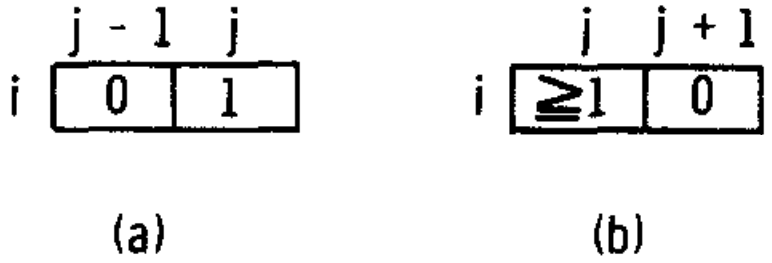
\includegraphics[keepaspectratio, width=6cm]{gambar/BorderFollowingPustaka/pic2.png}
			\caption{kondisi \textit{starting point} 
			dari algoritma \textit{border following} 
			untuk tepi luar (a) dan tepi lubang (b)}
			\label{gambar:kondisi_batas}
		\end{figure}
	\end{enumerate}
	\item Langkah 2 \\
	Tentukan \textit{parent border} untuk tepi piksel ($i,j$) 
	berdasarkan jenis tepi piksel dari piksel ($i,j$) dan LNBD
	(tepi terakhir yang ditemukan), mengikuti aturan pada tabel 
	(\ref{tabel:aturan_parent})
	\begin{table}[H]
		\caption{Aturan penetapan \textit{parent border}}
		\begin{tabular}[width=6cm]{| c | c | c |}
			\hline
			& \multicolumn{2}{|c|}
			{\textit{Type of border B' with the 
			sequentioal number of LNBD}} \\
			\hline
			\textit{Type of B} & \textit{Outer border} 
			& \textit{Hole border} \\
			\hline
			\textit{Outer border} & \textit{The parent border 
			of the border B'} & \textit{The border B'} \\
			\textit{Hole border} & \textit{The border B'} 
			&\textit{The parent border of the border B'} \\
			\hline
		\end{tabular}
		\label{tabel:aturan_parent}
	\end{table}
	\item langkah 3 \\
	Proses \textit{border following} dimulai dari 
	\textit{starting point} piksel ($i,j$) pada langkah ini
	\begin{enumerate}[(a)]
		\item Dimulai dari piksel ($i_2,j_2$), periksa piksel
		tetangga searah jarum jam dari piksel ($i,j$) sampai
		menemukan piksel \textit{non-zero}. Piksel \textit{non-zero}
		yang pertama ditemukan didefinisikan sebagai 
		($i_1,j_1$). jika piksel \textit{non-zero} tidak 
		ditemukan, set $f_{i,j} =$ -NBD dan lanjutkan ke langkah
		keempat
		\item $(i_2,j_2) \gets (i_1,j_1)$ dan
		$(i_3,j_3) \gets (i,j)$
		\item Mulai dari elemen setelah piksel($i_2,j_2$), mencari
		piksel \textit{non-zero} di sekitar piksel ($i_3,j_3$) 
		dengan arah berlawanan jarum jam dan set piksel 
		\textit{non-zero} pertama yang ditemukan ke dalam
		variabel ($i_4,j_4$).
		\item Ubah nilai $f_{i_3,j_3}$ dari piksel ($i_3,j_3$) 
		dengan aturan menandai(\textit{marking policy}):
		\begin{enumerate}[i]
			\item Jika piksel ($i_3,j_3+1$) 
			adalah 0-piksel (piksel bernilai 0), set
			$(i_3,j_3+1) \gets$ -NBD
			\item Jika piksel ($i_3,j_3+1$)  
			bukan 0-piksel (piksel bernilai 0), set
			$(i_3,j_3+1) \gets$ NBD
			\item Jika kedua kondisi di atas tidak terpenuhi,
			jangan ubah nilai $f_{i_3,j_3}$
		\end{enumerate}
		\item Jika $(i_4,j_4) = (i,j)$ dan $(i_3,j_3) = (i_1,j_1)$
		(kembali ke \textit{starting point}), maka lanjut ke 
		langkah 4, jika tidak set $(i_2,j_2) \gets (i_3,j_3)$, 
		$(i_3,j_3) \gets (i_4,j_4)$ dan kembali ke langkah (3.c).
	\end{enumerate}
	\item Langkah 4 \\
	jika $f_{i,j} \neq 1$, maka LNBD $\gets |f_{i,j}|$ dan
	lanjutkan pemindaian dari mulai piksel ($i,j+1$) 
	untuk kembali mencari nilai piksel objek $f_{i,j} \neq 0$.
	Algoritma dinyatakan selesai jika pemindai sudah sampai
	sudut kanan bawah dari citra(piksel terakhir)
\end{enumerate}
\begin{figure}[H]
	\centering
	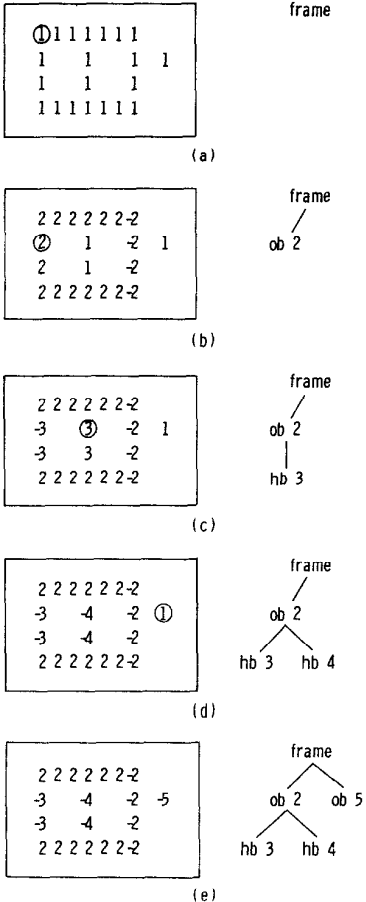
\includegraphics[keepaspectratio, width=7cm]{gambar/BorderFollowingPustaka/pic3.png}
	\caption{Ilustrasi proses pemberian hierarki terhadap piksel citra; 
	lingkaran pada piksel menunjukkan titik mula pindai \textit{border following}}
	\label{gambar:ProsesJalanBorderFollowing}
\end{figure}

\begin{figure}[H]
	\centering
	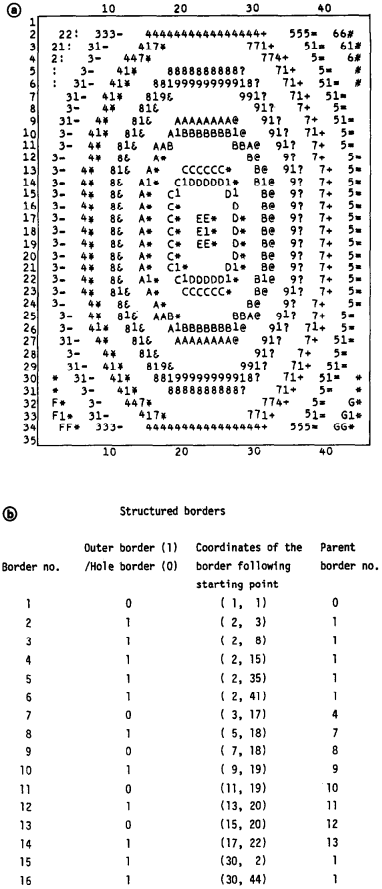
\includegraphics[keepaspectratio, width=9cm]{gambar/BorderFollowingPustaka/pic4.png}
	\caption{Struktur topologi antara tepi satu 
	dengan tepi yang lain jika menggunakan Algoritma 
	pertama. Hasil citra (a) dan Struktur yang diekstrak (b)}
	\label{gambar:Analisis_struktur_topologi}
\end{figure}

Selain algoritma pertama Suzuki, ia juga mengusulkan algoritma
kedua \textit{border following} di mana hasilnya hanya tepi 
terluarnya saja.Berikut perbedaan algoritma pertama dan 
algoritma kedua yang diusulkan Suzuki:
\begin{enumerate}
	\item Kondisi \textit{starting point} untuk melakukan
	operasi \textit{border following} hanya berlaku
	untuk tepi terluar (gambar \ref{gambar:kondisi_batas}) 
	dan jika LNBD $\leq 0$.
	\item \textit{Marking policy} tetap sama dengan algoritma
	pertama (langkah 3.d), tetapi nilai NBD dan -NBD akan
	diganti masing-masing dengan nilai 2 dan -2
	\item Nilai LNBD juga tetap disimpan dari piksel 
	\textit{non-zero} yang ditemukan sebelumnya. Akan
	tetapi, LNBD akan di-\textit{reset} ke nilai 0
	untuk setiap bari baru yang dipindai
\end{enumerate}

\begin{figure}[H]
	\centering
	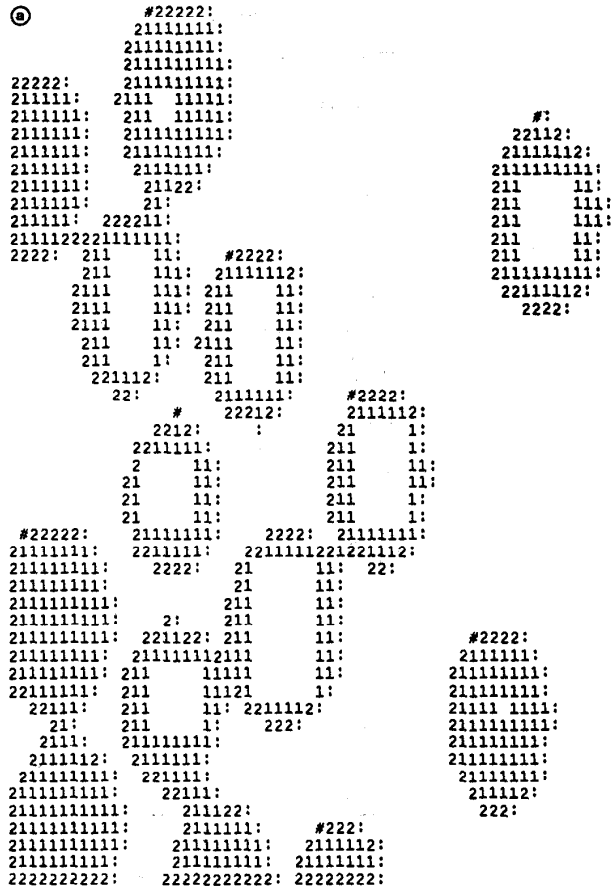
\includegraphics[keepaspectratio, width=8cm]{gambar/BorderFollowingPustaka/pic5.png}
	\caption{Hasil penciutan blob dengan 
	Algoritma kedua. “\#” merepresentasikan 
	\textit{starting point} dari tepi terluar, 
	“:” menunjukkan nilai -2.}
	\label{gambar:hasil_penciutan_blob}
\end{figure}

\section{\emph{Splines interpolation imaging}}

Pada konteks pengolahan citra, Interpolasi merupakan proses 
pembangunan kurva atau \textit{spline}, atau permukaan(\textit{surface}) terdefinisi 
bebas yang melalui sekumpulan titik data(\textit{data points}) 
secara tepat. Terkadang diberikan pembatas tambahan untuk 
mendapatkan interpolasi yang dibatasi agar mendapatkan hasil 
kurva atau \textit{spline} yang diinginkan(\cite{lockyer2006controlling}). \textit{Spline} 
yang sering dirujuk pada pengolahan citra adalah kurva yang 
dibentuk dengan gabungan polinominal. Contoh \textit{Spline} 
yang sudah di-interpolasikan dapat dilihat pada gambar (\ref{gambar:contohchordlength})


\subsection{\emph{Bézier Spline}}

Bézier \textit{Spline} merupakan salah satu kurva polinominal 
menggunakan kumpulan diskrit titik kontrol untuk 
membuat kurva yang halus dan kontinu. 

Bézier \textit{spline} dengan derajat ke-$n$ terdefinisikan 
sebagai berikut
\begin{equation}
	\begin{split}
		\textbf{C}(u) = \sum_{i = 0}^{n} B_{i,n}(u) \textbf{P}_i \quad
		& 0 \leq u \leq 1
	\end{split}
	\label{kurvabezier}
\end{equation}
Fungsi dasar (\textit{blending}), $\{B_{i,n}(u)\}$, merupakan 
polinominal Bernstein yang didefinisikan sebagai
\begin{equation}
	B_{i,n}(u) = \frac{n!}{i!(n-i)!} u^i (1-u)^{n-1}
	\label{bernstein}
\end{equation}
Koefisien geometri dalam bentuk ini, $\{\textbf{P}_i\}$, disebut 
sebagai titik kontrol(\textit{control points}), dan pada 
persamaan (\ref{kurvabezier}), $u$ nya harus diantara 0 sampai 1 
$[u \in [0,1]]$

Bisa dicontohkan hasil Bézier sebagai berikut. Bézier 
memiliki derajat 2, $n = 2$, tarik dari persamaan 
(\ref{kurvabezier}) dan (\ref{bernstein}), bisa didapat
$\textbf{C}(u) = (1 - u)^2 \textbf{P}_0 + 2u(1 - u) 
\textbf{P}_1 + u^2 \textbf{P}2$ akan menghasilkan 
busur parabola dari $\textbf{P}_0$ ke $\textbf{P}_2$. 
Dapat kita lihat pada gambar(\ref{gambar:Bezier_derajat2})
\begin{itemize}
	\item poligon yang dibentuk oleh 
	$\{\textbf{P}_0, \textbf{P}_1, \textbf{P}_2\}$, 
	disebut sebagai \textit{control polygon}, mendekati 
	bentuk kurva yang cukup baik.
	\item $\textbf{P}_0 = \textbf{C}(0)$ dan 
	$\textbf{P}_2 = \textbf{C}(1)$.
	\item arah tangen kepada kurva yang berada di titik akhir 
	paralel terhadap $\textbf{P}_1 - \textbf{P}_0$ dan 
	$\textbf{P}_2 - \textbf{P}_1$.
	\item kurva berada di dalam segitiga yang dibentuk 
	$\textbf{P}_0\textbf{P}_1\textbf{P}_2$
\end{itemize}
\begin{figure}[H]
	\centering
	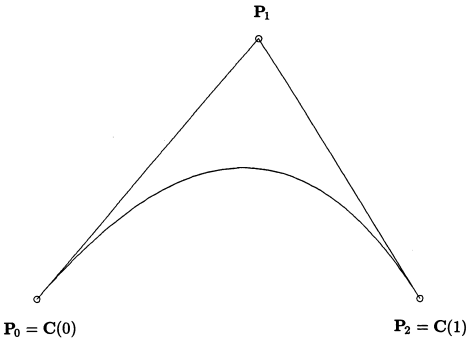
\includegraphics[keepaspectratio, width=10cm]{gambar/Interpolasi/bezierderajat2.png} 
	\caption{Kurva Bézier berderajat-2.}
	\label{gambar:Bezier_derajat2}
\end{figure}


\subsection{\emph{B-Spline}}

pada analisis numerik dalam matematika, 
\textit{B-Spline} atau bisa disebut dengan 
\textit{basis spline} merupakan fungsi spline dengan 
tunjangan yang sedikit dengan diberikan derajat, kehalusan, 
dan partisi domain.
Kurva yang hanya berisikan satu polinomial atau 
segmentasi rasional yang sering tidak memadai, 
kekurangannya adalah:
\begin{itemize}
	\item memerlukan \textit{high degree}(interpolasi 
	dengan derajat tinggi) untuk kompensasi  
	banyak keterbatasan; misalnya, ($n - 1$)-derajat 
	diperlukan untuk melewatkan kurva Bézier polinomial 
	melalui $n$ titik data. Namun, kurva tingkat tinggi 
	tidak efisien untuk diproses dan secara numerik tidak stabil;
	\item Suatu \textit{high degree} diperlukan untuk 
	\textit{fitting} bentuk(formula) kompleks secara akurat
	\item kurva segment tunggal (\textit{surface} atau 
	disebut permukaan) tidak cocok untuk desain 
	bentuk(formula) interaktif; meskipun kurva Bézier dapat 
	dibentuk melalui titik kontrolnya (dan bobot), 
	kontrolnya tidak cukup lokal.
\end{itemize}

Solusinya adalah dengan menggunakan kurva (atau permukaan) 
yang \textit{piecewise polynomial}(polinomial yang dipotong-potong), 
atau \textit{piecewise rational}(rasional yang dipotong-potong). 
Gambar (\ref{gambar:Kurva_dipotong_tiga}) 
menunjukkan kurva $\textbf{C}(u)$, yang terdiri 
dari $m$ (= 3) segmen polinomial  berderajat-$n$. 
$\textbf{C}(u)$ didefinisikan pada $u\in$ [0, 1]. 
Nilai parameter $u_0 = 0 < u_1 < u_2 < u_3$ = 1 disebut 
\textit{breakpoints}. Mereka memetakan ke titik akhir dari 
tiga segmen polinomial. ditunjukkan segmen 
sebagai $\textbf{C}_{i}(u)$, $1 \leq i \leq m$. 
Segmen-segmen tersebut 
dibangun sedemikian rupa sehingga bergabung dengan 
tingkat kontinuitas tertentu (tidak harus sama di 
setiap \textit{breakpoint}). Misalkan 
$\textbf{C}_{i}^{(j)}$ menyatakan 
turunan ke-$j$ dari $\textbf{C}_i$. $\textbf{C}(u)$ 
dikatakan $\textbf{C}^k$ kontinu pada \textit{breakpoint} 
$u_i$ jika $\textbf{C}_{i}^{(j)}(u_i) = C_{i+1}^{(j)}(u_i)$ 
untuk semua $0 \leq j \leq k$.
\begin{figure}[H]
	\centering
	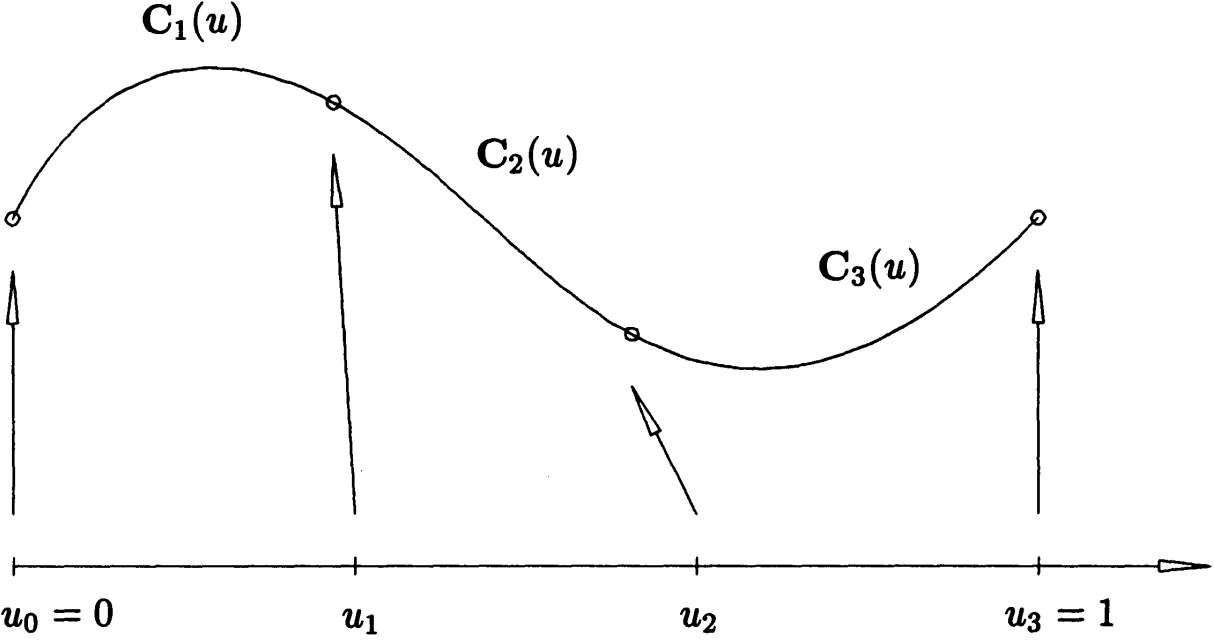
\includegraphics[keepaspectratio, width=10cm]{gambar/Interpolasi/pic1.png} 
	\caption{Kurva polinomial kubik dipotong tiga segmen.}
	\label{gambar:Kurva_dipotong_tiga}
\end{figure}

Setiap bentuk polinomial standar dapat digunakan 
untuk menyatakan bentuk $\textbf{C}_{i}(u)$. 
Gambar (\ref{gambar:Kurva_dipotong_tiga_dipotong_lagi}) 
menunjukkan kurva Gambar (\ref{gambar:Kurva_dipotong_tiga}) 
dengan tiga segmen  dalam bentuk kubik Bézier. 
$\textbf{P}_i^j$ menunjukkan titik kontrol ke-$i$ dari segmen ke-$j$.
\begin{figure}[H]
	\centering
	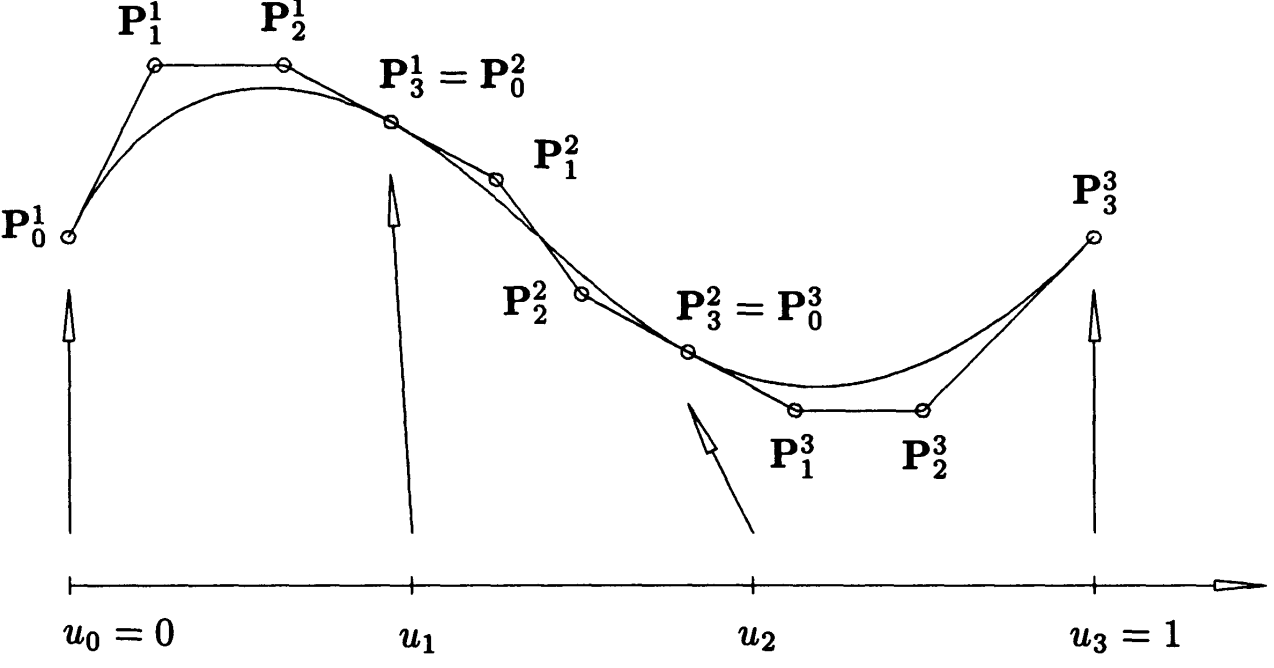
\includegraphics[keepaspectratio, width=10cm]{gambar/Interpolasi/pic2.png} 
	\caption{Kurva Gambar (\ref{gambar:Kurva_dipotong_tiga}) 
	ditunjukkan dengan segmen polinomial yang direpresentasikan 
	dalam bentuk Bézier.}
	\label{gambar:Kurva_dipotong_tiga_dipotong_lagi}
\end{figure}

Jika derajatnya sama dengan tiga dan \textit{breakpoints} 
$U = {u_0, u_1, u_2, u_3}$ tetap, dan jika dua 
belas titik kontrol, $\textbf{P}_i^j $, bervariasi 
secara sembarangan, akan memperoleh ruang vektor, $\nu$, 
yang terdiri dari semua potongan kurva polinomial 
kubik di $U$. $\nu$ memiliki dimensi dua belas, dan kurva 
di $\nu$ mungkin terputus-putus di $u_1$ atau $u_2$. 
Sekarang misalkan ditetapkan (seperti pada 
Gambar (\ref{gambar:Kurva_dipotong_tiga_dipotong_lagi})) 
bahwa $\textbf{P}_3^1 = \textbf{P}_0^2$ 
dan $\textbf{P}_3^2 = \textbf{P}_0^3$. Hal ini 
akan menghasilkan $\nu^0$, ruang vektor dari semua 
potongan kurva polinomial kubik pada $U$ yang 
setidaknya $\textbf{C}^0$ kontinu di semua titik. $\nu^0$ memiliki 
dimensi sepuluh, dan $\nu^0 \subset \nu$

Dari paragraf di atas, bisa dibuat kurva yang 
representatif dalam bentuk:

\begin{equation}
	\textbf{C}(u) = \sum_{i = 0}^{n} f_{i}(u) \textbf{P}_i
	\label{rumusdasarB}
\end{equation}
\begin{itemize}
	\item $\textbf{P}_i$ adalah titik kontrol
	\item {$f_{i}(u), i = 0$, ..., $n$} adalah 
	potongan fungsi polinomial yang membentuk 
	basis untuk ruang vektor semua fungsi potongan 
	polinomial dengan derajat dan kontinuitas yang 
	diinginkan (untuk sebuah urutan breakpoint tetap, 
	$U = {u_i}$, $0 \leq i \leq m$)
\end{itemize}
Perhatikan bahwa kontinuitas ditentukan oleh 
fungsi basis\textit{basis function}, sehingga 
titik kontrol dapat dimodifikasi tanpa mengubah 
kontinuitas kurva. Selain itu, {$f_i$} harus memiliki 
sifat analitik bagus yang 'biasa'. Hal ini 
memastikan bahwa kurva yang ditentukan oleh 
Persamaan (\ref{rumusdasarB}) memiliki sifat 
geometri yang mirip dengan kurva Bézier, misalnya 
\textit{convex hull}, \textit{variation diminishing}, 
\textit{transformation invariance}. Properti penting 
lainnya yang dicari dalam fungsi basis ini adalah \textit{local support}; 
ini menyiratkan bahwa setiap $f_{i}(u)$ bukan nol 
hanya pada sejumlah subinterval yang terbatas, 
bukan seluruh domain, [$u_0$, $u_m$]. Karena $\textbf{P}_i$ 
dikalikan dengan $f_{i}(u)$, pergerakan $\textbf{P}_i$ 
mempengaruhi bentuk kurva hanya pada subinterval 
di mana $f_{i}(u)$ bukan nol.

Ada banyak cara untuk mendefinisikan $f_{i}(u)$ 
pada rumus (\ref{rumusdasarB}), di sini akan memakai 
cara \textit{recurrence formula}. Misalkan $U = {u_0, \dots, um}$ 
adalah barisan bilangan real tak menurun, yaitu 
$u_i \leq u_i+1$, $i = 0, \dots, m - 1$. $u_i$ disebut 
\textit{knots}, dan $U$ adalah \textit{knots vector}. 
Fungsi basis \textit{B-spline} ke-$i$ merupakan $p$-derajat 
(ordo $p+l$), dilambangkan dengan $N_{i,p}(u)$, 
didefinisikan sebagai
\begin{equation}
	\begin{split}
	&N_{i,0}(u) = \begin{cases}
		1 \quad \text{if} \quad u_i \leq u < u_{i+1} \\
		0 \quad \text{otherwise}
	\end{cases}
	\\
	&N_{i,p}(u) = \frac{u - u_i}{u_{i+p} - u_i}N_{i,p-1}(u) + \frac{u_{i+p+1} - u}{u_{i+p+1} - u_{i+1}}N_{i+1,p-1}(u)
	\label{rumusdasarN}
	\end{split}
\end{equation}
Dengan catatan :
\begin{itemize}
	\item $N_{i,0}(u)$ merupakan fungsi langkah(\textit{step function})
	yang hampir semua hasilnya merupakan nol kecuali 
	di dalam interval setengah terbuka $u \in [ui, u{i+1})$
	\item Untuk $p > 0, N_{i,p}(u)$ merupakan kombinasi 
	linear dari dua fungsi dasar ($p$ - 1)-derajat. 
	(gambar \ref{gambar:definisirumusdasar})
	\begin{figure}[H]
		\centering
		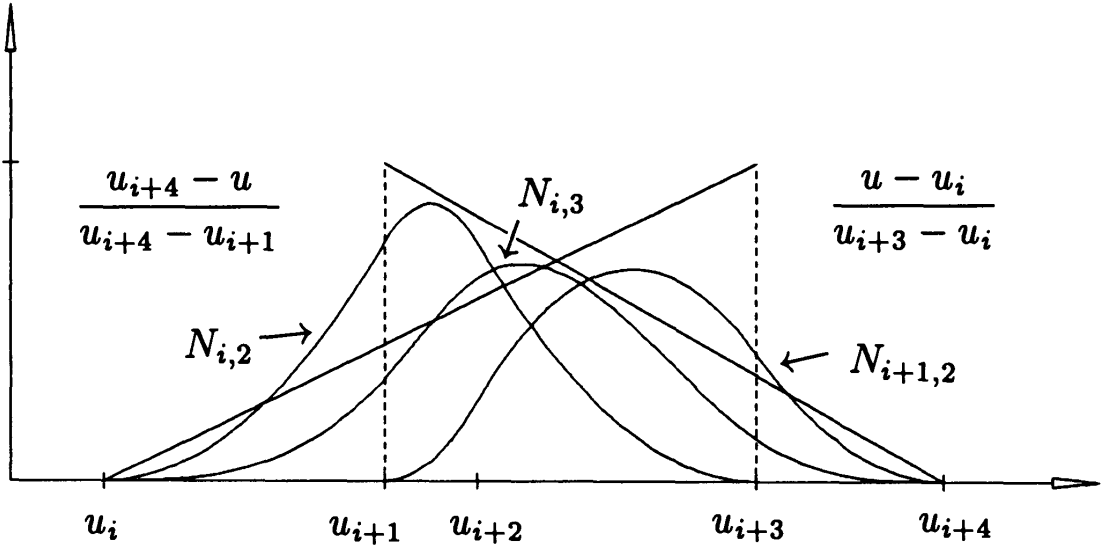
\includegraphics[keepaspectratio, width=10cm]{gambar/Interpolasi/pic3.png}
		\caption{definisi rekursif dari rumus dasar B-spline.}
		\label{gambar:definisirumusdasar}
	\end{figure}
	\item Komputasi dari kumpulan fungsi dasar 
	memerlukan spesifikasi dari sebuah \textit{knot vector}, 
	$U$, dan derajatnya, $p$.
	\item Rumus (\ref{rumusdasarN}) bisa menghasilkan 0/0; 
	nanti hasilnya diubah menjadi nol.
	\item $N_{i,p}(u)$ adalah potongan polinomial, 
	yang didefinisikan pada seluruh garis ril; umumnya 
	hanya pada interval [$u_0$, $u_m$] yang diperhatikan.
	\item interval setengah terbuka, [$u_i, u_{i+1}$), disebut 
	\textit{knot span} ke-$i$; panjangnya bisa nol, 
	karena \textit{knot} tidak perlu dibedakan;
	\item perhitungan fungsi derajat ke-$p$ 
	menghasilkan tabel segitiga terpotong \\
	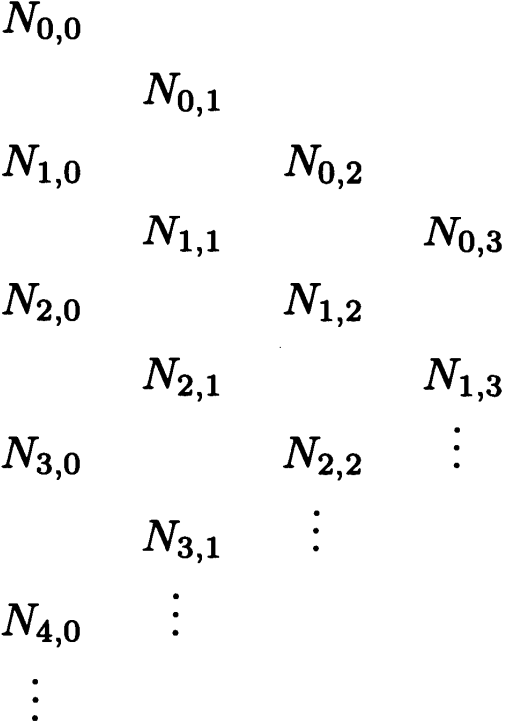
\includegraphics[keepaspectratio, width=4cm]{gambar/Interpolasi/pic4.png}
\end{itemize}

Dengan seluruh hal di atas, penulis mendapatkan 
rumus dasar untuk merubah suatu kurva acak menjadi 
kurva yang memiliki kontinuitas. Bahasan berikut akan 
menyempurnakan rumus dasar untuk memiliki kontinuitas 
yang lebih lanjut.

\subsection{\emph{Global Interpolation}}

Kebanyakan algoritma interpolasi terbagi dalam 
salah satu dari dua kategori: global atau lokal. 
Dengan algoritma global, sistem masalah pada persamaan 
atau optimasi sudah diatur dan diselesaikan. Jika 
data yang diberikan hanya terdiri dari titik dan 
turunan, dan jika yang tidak diketahui hanya 
titik kontrol (derajat, \textit{knot}, dan 
bobot telah dipilih sebelumnya), maka sistem tersebut 
linier dan karenanya akan mudah diselesaikan. Jika data 
yang lebih esoterik, seperti kelengkungan diketahui, 
atau \textit{knot} dan/atau bobot juga tidak diketahui sistemnya, 
maka sistem yang dihasilkan adalah nonlinier. Secara 
teoritis, gangguan pada \textit{input item data} 
siapa pun dapat mengubah bentuk keseluruhan kurva 
atau permukaan; namun, besarnya perubahan menurun 
seiring bertambahnya jarak dari \textit{item data} 
yang terpengaruh. Algoritma lokal lebih bersifat 
geometris, membangun kurva atau segmen permukaan, 
hanya menggunakan data lokal untuk setiap langkah. 
Gangguan pada item data hanya mengubah kurva atau 
permukaan secara lokal. Algoritme ini biasanya lebih 
murah secara komputasi dibandingkan metode global. 
Mereka juga dapat menangani titik puncak, segmen garis 
lurus, dan anomali data lokal lainnya dengan lebih baik. 
Namun, mencapai tingkat kontinuitas yang diinginkan 
pada batas segmen lebih menyusahkan, dan metode lokal 
sering kali menghasilkan banyak \textit{interior knot}.

Berikut merupakan pembentukan rumus interpolasi global.
Misalkan penulis diberikan sekumpulan titik {$\textbf{Q}_k$}, 
$k$ = 0, ..., $n$, dan penulis ingin menginterpolasi 
titik-titik ini dengan kurva \textit{B-spline} 
nonrasional $p$-derajat. Jika ditetapkan nilai 
parameter, $\bar{u}k$, pada masing-masing $\textbf{Q}_k$, 
dan memilih \textit{knot vector} yang sesuai $U = {u_0, ..., u_m}$, 
dapat disiapkan sistem persamaan linier 
(n + 1) variabel dan (n + 1) persamaan:
\begin{equation}
	\textbf{Q}_k = \textbf{C}(u) = \sum_{i = 0}^{n} N_{i,p}(\bar{u}_k) \textbf{P}_i
	\label{rumus:Global}
\end{equation}
Titik kontrol, $\textbf{P}_i$, adalah variabel $n$ + 1 yang 
tidak diketahui. $r$ merupakan jumlah koordinat 
dalam $\textbf{Q}_k$ (biasanya 2, 3, atau 4). 
Perhatikan bahwa metode ini tidak bergantung pada $r$; 
Persamaan (\ref{rumus:Global}) mempunyai satu koefisien 
matriks, dengan $r$ sisi kanan dan, dengan demikian, 
$r$ merupakan himpunan solusi untuk $r$ koordinat dari $\textbf{P}_i$.

Masalah berada dalam pemilihan $\bar{u}_k$ dan $U$, 
dan pilihannya mempengaruhi bentuk dan parameterisasi 
kurva. Sepanjang bagian ini diasumsikan bahwa 
parameternya terletak pada rentang $U \in [0, 1]$. 
Tiga metode umum dalam memilih $\bar{u}_k$ adalah:
\begin{itemize}
	\item \textit{equally spaced}: \\
	\begin{equation}
		\begin{split}
			\bar{u}_0 = 0 \quad & \bar{u}_n = 1 \\
			\bar{u}_k = \frac{k}{n} \quad & k = 1, ..., n-1
		\end{split}
		\label{rumus:equallyspaced}
	\end{equation}
	Metode ini tidak direkomendasikan dikarenakan 
	bisa membuat bentuk yang tak menentu (seperti \textit{loops}) 
	ketika datanya tidak berjarak sama

	\item \textit{chord length}: diumpamakan $d$ 
	merupakan jumlah chord length
	\begin{equation}
		d = \sum_{k=1}^{n}|\textbf{Q}_k - \textbf{Q}_{k-1}|
		\label{chordlength1}
	\end{equation}
	lalu \centerline {\quad $\bar{u}_0 = 0$ \quad $\bar{u}_n = 1$}
	\begin{equation}
		\bar{u}_k = \bar{u}_{k-1} + \frac{|\textbf{Q}_k - \textbf{Q}_{k-1}|}{d} \quad
		k = 1, ..., n-1
		\label{chordlength2}
	\end{equation}
	Ini adalah metode yang paling banyak digunakan, 
	dan secara umum sudah memadai. Hal ini juga 
	memberikan parameterisasi yang "bagus" pada 
	kurva, dalam arti mendekati parameterisasi 
	yang seragam.

	\item metode \textit{centripetal}: umpamakan
	\[d = \sum_{k=1}^{n} \sqrt{|\textbf{Q}_k - \textbf{Q}_{k-1}|} \]
	lalu \centerline {\quad $\bar{u}_0 = 0$ \quad $\bar{u}_n = 1$}
	\begin{equation}
		\bar{u}_k = \bar{u}_{k-1} + \frac{\sqrt{|\textbf{Q}_k - \textbf{Q}_{k-1}|}}{d} \quad
		k = 1, ..., n-1
		\label{centripetal}
	\end{equation}
\end{itemize}

\textit{Knots} bisa berjarak sama, yaitu:
\begin{equation}
	\begin{split}
		u_0 = ... = u_p = 0 \qquad & u_{m-p} = ... = u_m = 1 \\
		u_{j+p} = \frac{j}{n-p+1} \qquad & j = 1, ..., n-p
	\end{split}
	\label{penjarakanknots}
\end{equation}
Namun, cara ini tidak disarankan, jika digunakan 
bersama dengan Persamaan (\ref{chordlength2}) 
atau (\ref{centripetal}) dapat menghasilkan sistem 
persamaan tunggal pada Persamaan \ref{rumus:Global}. 
untuk mengatasinya ada teknik rata-rata sebagai berikut
\begin{equation}
	\begin{split}
		u_0 = ... = u_p = 0 \qquad & u_{m-p} = ... = u_m = 1 \\
		u_{j+p} = \frac{1}{p}\sum_{i=j}^{j+p-1}\bar{u}_i \qquad & j = 1, ..., n-p
	\end{split}
	\label{penjarakanrata_rataknots}
\end{equation}
Dengan metode ini knots mencerminkan distribusi 
$\bar{u}_k$. Selanjutnya menggunakan Persamaan (\ref{penjarakanrata_rataknots}) 
dikombinasikan dengan Persamaan (\ref{chordlength2}) 
atau (\ref{centripetal}) untuk menghitung $\bar{u}_k$ 
mengarah ke sistem (Persamaan \ref{rumus:Global}) 
yang benar-benar positif dan terikat dengan 
\textit{semibandwidth} kurang dari $p$, yaitu, 
$N_{i,p}(\bar{u}_k) = 0$ jika $|i - k| \geq p$. 
Oleh karena itu, penyelesaiannya dapat dilakukan 
dengan eliminasi Gaussian tanpa melakukan \textit{pivoting}.

\begin{figure}[H]
	\centering
	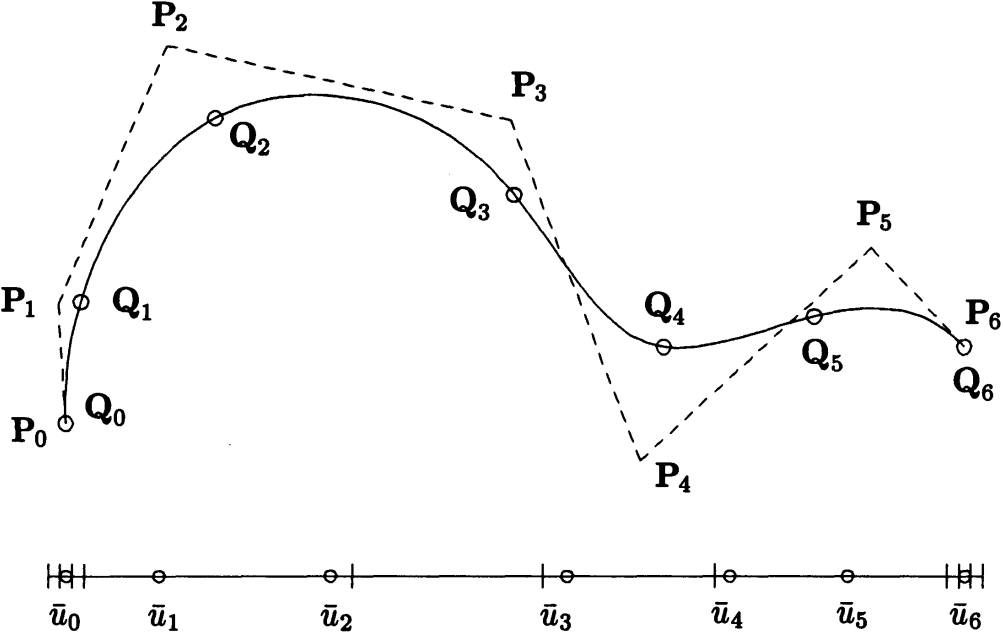
\includegraphics[keepaspectratio, width=10cm]{gambar/Interpolasi/pic5.png}
	\caption{Contoh interpolasi kurva menggunakan 
	parameterisasi \textit{chord length} dan \textit{knot vector}  
	yang diperoleh dengan rata-rata parameter.}
	\label{gambar:contohchordlength}
\end{figure}

Gambar (\ref{gambar:contohchordlength}) menunjukkan titik kontrol, parameter, 
dan \textit{knot vector} dari kurva kubik yang menginterpolasi 
tujuh titik. Parameter ditentukan dengan metode 
\textit{chord length}, dan \textit{knot} diperoleh 
dengan merata-ratakan parameternya (Persamaan \ref{penjarakanrata_rataknots}). 
Pada Gambar (\ref{gambar:interpolasi1}) diilustrasikan perbandingan 
parameterisasi yang berbeda. Gambar 
(\ref{gambar:interpolasi2}) menunjukkan 
perbandingan yang sama dengan menggunakan lebih banyak 
titik data yang tersebar secara "liar". Dalam kedua 
kasus tersebut, kurva kubik dilewatkan melalui tujuh 
titik, menggunakan parameter seragam dan knot seragam 
(kurva padat dan knot vector atas - lihat Persamaan 
[\ref{rumus:equallyspaced}] dan [\ref{penjarakanknots}]); 
parameter \textit{chord length} dan \textit{knot} yang diperoleh 
dengan rata-rata (kurva putus-putus dan \textit{knot vector} 
tengah - lihat Persamaan [\ref{chordlength2}] dan 
[\ref{penjarakanrata_rataknots}]); dan parameter 
sentripetal serta knot yang diperoleh dengan 
rata-rata (kurva titik-titik dan knot vector 
bawah - lihat Persamaan [\ref{centripetal}] dan 
[\ref{penjarakanrata_rataknots}]). Perhatikan akan 
Gambar (\ref{gambar:interpolasi2}) bagaimana 
\textit{chord length} dan kurva 
parameter sentripetal beradaptasi dengan perubahan 
jarak titik.

\begin{figure}[H]
	\centering
	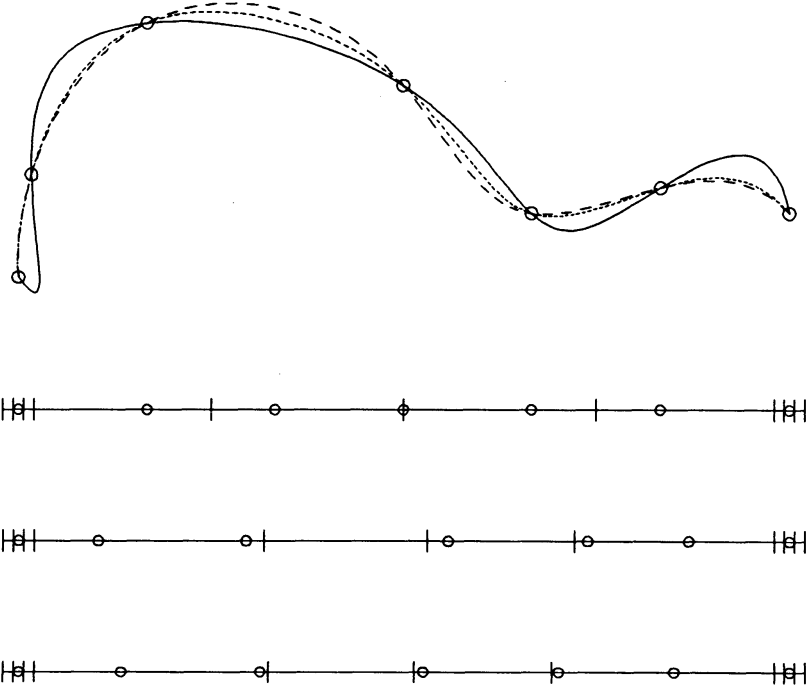
\includegraphics[keepaspectratio, width=10cm]{gambar/Interpolasi/pic6.png}
	\caption{Contoh interpolasi kurva dengan 
	parameterisasi dan \textit{knot vector}  berbeda.}
	\label{gambar:interpolasi1}
\end{figure}

\begin{figure}[H]
	\centering
	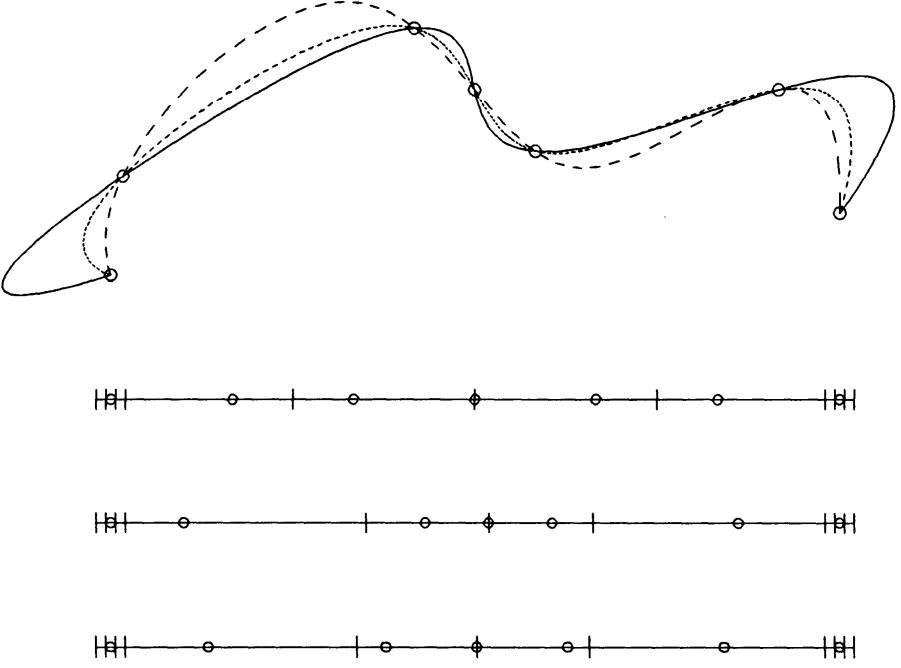
\includegraphics[keepaspectratio, width=10cm]{gambar/Interpolasi/pic7.png}
	\caption{Contoh interpolasi kurva dengan 
	parameterisasi dan \textit{knot vector}  berbeda.}
	\label{gambar:interpolasi2}
\end{figure}

Gambar (\ref{gambar:interpolasi3}) mengilustrasikan 
interpolasi dengan derajat yang berbeda-beda; 
kurva padat, putus-putus, dan putus-putus 
masing-masing memiliki derajat 2, 3, dan 4. 
Gambar (\ref{gambar:interpolasi4}) menunjukkan 
ketidakmampuan interpolasi global untuk menangani 
kumpulan titik kolinear.

\begin{figure}[H]
	\centering
	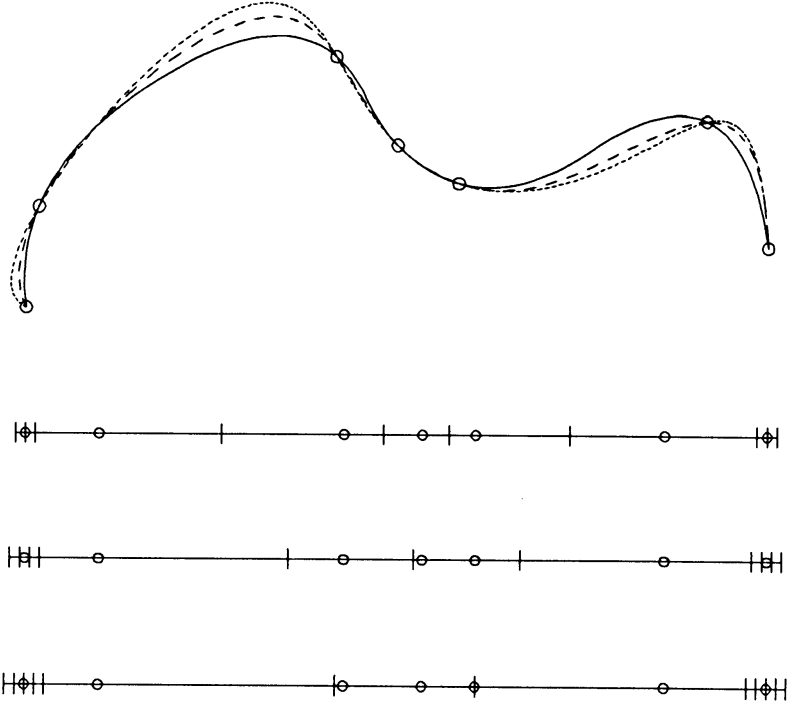
\includegraphics[keepaspectratio, width=10cm]{gambar/Interpolasi/pic8.png}
	\caption{Interpolasi kurva dengan derajat 
	berbeda menggunakan parameterisasi chord 
	length dan knot yang diperoleh dengan rata-rata.}
	\label{gambar:interpolasi3}
\end{figure}

\begin{figure}[H]
	\centering
	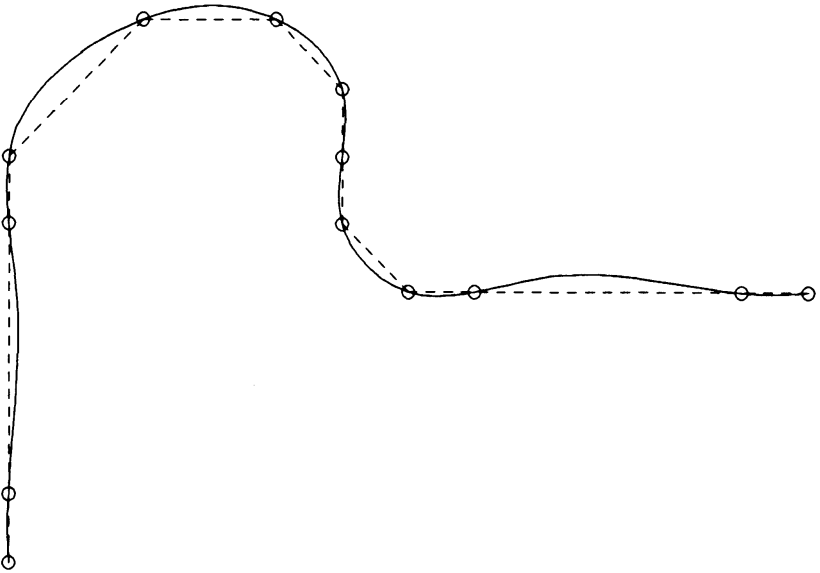
\includegraphics[keepaspectratio, width=10cm]{gambar/Interpolasi/pic9.png}
	\caption{Interpolasi kurva kubik global 
	ke data yang berisi titik-titik kolinear 
	(lihat garis putus-putus).}
	\label{gambar:interpolasi4}
\end{figure}
Setelah $\bar{u}_k$ dan \textit{knot} dihitung, matriks koefisien 
$(n+1)$ x $(n+1)$ dari sistem (Persamaan \ref{rumus:Global}) 
dibuat dengan mengevaluasi fungsi basis bukan nol pada 
setiap $\bar{u}_k, k = 0, . ..., n$.

\textbf{Contoh:}

Misalkan {$\textbf{Q}_k$} = {(0, 0), (3, 4), (-1, 4), 
(-4, 0), (-4, -3)}, dan asumsikan penulis ingin 
menginterpolasi $\textbf{Q}_k$ dengan kurva kubik. 
Digunakan persamaan (\ref{chordlength2}) dan 
(\ref{penjarakanrata_rataknots}) untuk menghitung 
$\bar{u}_k$ dan $u_j$, dan kemudian membuat sistem persamaan 
linier, Persamaan (\ref{rumus:Global}). \textit{chord lengths} 
yang terpisah adalah

\centerline{$|\textbf{Q}_1 - \textbf{Q}_0| = 5$ \quad
$|\textbf{Q}_2 - \textbf{Q}_1| = 4$ \quad
$|\textbf{Q}_3 - \textbf{Q}_2| = 5$ \quad
$|\textbf{Q}_4 - \textbf{Q}_3| = 3$}

Dan jumlah \textit{chord length} menjadi $d = 17$, maka

\centerline{$\bar{u}_0 = 0$ \quad
$\bar{u}_1 = \frac{5}{17}$ \quad
$\bar{u}_2 = \frac{9}{17}$ \quad
$\bar{u}_3 = \frac{14}{17}$ \quad
$\bar{u}_4 = 1$}
Gunakan rumus (\ref{penjarakanrata_rataknots})
\[u_4 = \frac{1}{3}(\frac{5}{17}+\frac{9}{17}+\frac{14}{17})=\frac{28}{51} \]
maka \[U = \{0,0,0,0,\frac{28}{51},1,1,1,1\}\]
Sistem persamaan linearnya adalah
\[ \begin{split}
	\begin{bmatrix}
	1 & 0 & 0 & 0 & 0\\ 
	N_{0,3}(\frac{5}{17}) & N_{1,3}(\frac{5}{17}) & N_{2,3}(\frac{5}{17}) & N_{3,3}(\frac{5}{17}) & 0\\ 
	N_{0,3}(\frac{9}{17}) & N_{1,3}(\frac{9}{17}) & N_{2,3}(\frac{9}{17}) & N_{3,3}(\frac{9}{17}) & 0\\ 
	0 & N_{1,3}(\frac{14}{17}) & N_{2,3}(\frac{14}{17}) & N_{3,3}(\frac{14}{17}) & N_{4,3}(\frac{14}{17})\\ 
	0 & 0 & 0 & 0 & 1
	\end{bmatrix} &
	\begin{bmatrix}
		\textbf{P}_0 \\
		\textbf{P}_1 \\
		\textbf{P}_2 \\
		\textbf{P}_3 \\
		\textbf{P}_4 
	\end{bmatrix}
	\\
	= & \begin{bmatrix}
		\textbf{Q}_0 \\
		\textbf{Q}_1 \\
		\textbf{Q}_2 \\
		\textbf{Q}_3 \\
		\textbf{Q}_4
	\end{bmatrix}
	\end{split}
\]

\subsection{\emph{Local Interpolation}}

Seperti yang dikatakan sebelumnya, interpolasi global 
tidak memberikan hasil yang sempurna, karena rumus nya terlalu 
mengeneralisir pemindahan \textit{knot vector}. 
Untuk mengatasi hal itu, 
digunakan interpolasi lokal. Misalkan {$Q_k$} , $k = 0, ..., n$, 
diberikan. Yang dimaksud dengan interpolasi kurva lokal adalah 
metode yang membentuk $n$ segmen kurva polinomial atau rasional, 
$C_{i}(u), i = 0, ..., n - 1$, sehingga $Q_i$ dan $Q_{i+1}$ 
adalah titik akhir dari $C_{i}(u)$. Segmen-segmen yang 
berdekatan digabungkan dengan tingkat kontinuitas 
tertentu, dan konstruksi berlangsung berdasarkan segmen, 
umumnya dari kiri ke kanan. Persamaan apa pun yang muncul 
bersifat lokal hanya pada beberapa segmen yang berdekatan. 
Dalam \textit{framework} NURBS, mereka membuat segmen menggunakan 
kurva Bézier polinomial atau rasional, kemudian memperoleh 
kurva NURBS dengan memilih \textit{knot vector} yang sesuai.

\begin{figure}[H]
	\centering
	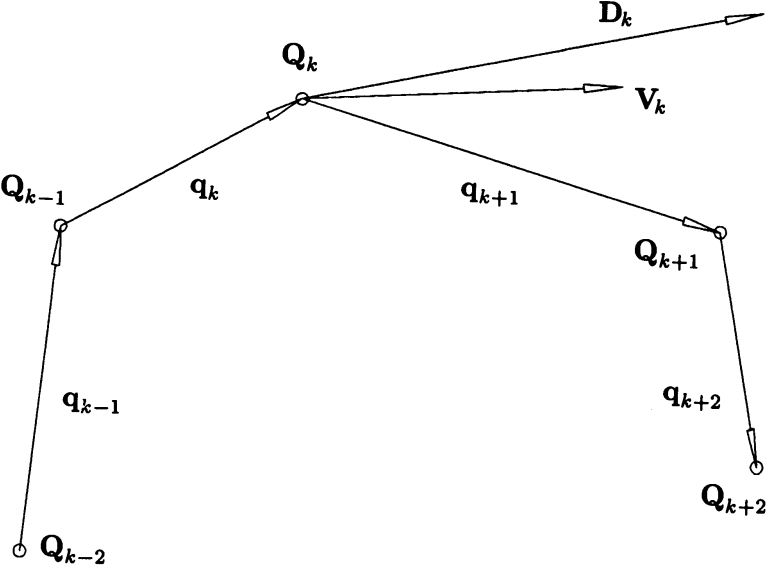
\includegraphics[keepaspectratio, width=10cm]{gambar/Interpolasi/pic10.png}
	\caption{Perhitungan vektor tangen ($\textbf{V}_k$) dan 
	turunan ($\textbf{D}_k$) untuk interpolasi kurva lokal.}
	\label{gambar:arahtangendanturunan}
\end{figure}

Sekarang misalkan $\bar{u}_i$ menyatakan parameter awal 
$\textbf{C}_{i}(u)$ dan parameter akhir $\textbf{C}_{i-1}(u)$. 
$\textbf{C}_{i}(u)$ dan $\textbf{C}_{i-1}(u)$. bertemu di 
$\bar{u}_i$ dengan kontinuitas $G^1$ (G untuk geometri) 
jika arah singgungnya berimpit di sana, yaitu jika 
$\textbf{C}'_{i}(\bar{u}_i)$ dan $\textbf{C}'_{i-1}(\bar{u}_i)$ 
menunjuk ke arah yang sama. Namun, besarnya mungkin berbeda. 
Kontinuitas $G^1$ menyiratkan bahwa kurva tersebut 
secara visual kontinu (halus) tetapi mungkin memiliki 
diskontinuitas dalam parameterisasinya. Algoritma 
interpolasi lokal dirancang untuk memberikan tingkat 
kontinuitas $G$ atau $C$ tertentu; dalam sub bab ini 
hanya menyajikan algoritma yang menyediakan 
kontinuitas $G^1$ atau $C^1$. Metode lokal yang 
menghasilkan kontinuitas lebih tinggi tidak 
banyak digunakan. Meskipun $G^2$ dan $C^2$ dimungkinkan 
dengan kubik, derajat yang lebih tinggi harus 
digunakan jika fleksibilitas yang wajar ingin dipertahankan.

Untuk mendapatkan segmen Bézier, $\textbf{C}_{i}(u)$, 
memerlukan komputasi titik kontrol Bézier bagian dalam, 
satu titik untuk kuadrat, dua untuk kubik. Titik kendali 
ini terletak pada garis singgung(\textit{tangent}) kurva di 
$\textbf{Q}_k$; oleh karena itu, diperlukan vektor 
singgung(\textit{tangent vector}) $\textbf{T}_k$ pada 
setiap $\textbf{Q}_k$. Dalam beberapa kasus, vektor 
tersebut dapat dimasukkan bersama dengan $\textbf{Q}_k$; 
misalnya, persamaan tersebut mudah diperoleh saat 
menghitung titik potong antara dua permukaan. Namun, 
jika tidak dimasukkan maka harus dihitung sebagai bagian 
dari algoritma interpolasi. Ada sejumlah metode; Boehm 
[\cite{BOHM19841}] memberikan survei tentang berbagai 
metode. Misalkan
\[\Delta\bar{u}_k = \bar{u}_k - \bar{u}_{k-1} \quad
\textbf{q}_k = \textbf{Q}_k - \textbf{Q}_{k-1} \quad
\textbf{d}_k = \frac{\textbf{q}_k}{\Delta\bar{u}_k}
\]
Semua metode memiliki satu dari dua bentuk
\begin{equation}
	\textbf{D}_k = (1 - \alpha_k)\textbf{d}_k = \alpha_{k}\textbf{d}_{k+1}
	\label{rumus:turunanlokal} 
\end{equation}
atau
\begin{equation}
	\textbf{T}_k = \frac{\textbf{V}_k}{|\textbf{V}_k|} \quad
	\textbf{V}_k = (1 - \alpha_k)\textbf{q}_k + \alpha_{k}\textbf{q}_{k+1}
	\label{rumus:tangenlokal} 
\end{equation}
(lihat Gambar \ref{gambar:arahtangendanturunan}). 
Perhatikan bahwa Persamaan (\ref{rumus:turunanlokal}) 
mengasumsikan bahwa nilai $\bar{u}_k$ telah ditetapkan. 
Vektor $\textbf{D}_k$ dapat dipandang sebagai perkiraan 
turunannya. Persamaan (\ref{rumus:tangenlokal}) tidak 
menggunakan parameter $\bar{u}_k$ dan vektor yang 
dihasilkan harus dipandang sebagai arah singgung saja. 
Penetapan besaran dan parameter harus dilakukan bersamaan 
satu sama lain karena tidak independen. Perhatikan 
juga bahwa ini menggunakan notasi $\textbf{T}$ hanya 
untuk vektor singgung satuan panjang. Persamaan 
(\ref{rumus:turunanlokal}) dan (\ref{rumus:tangenlokal}) 
merupakan interpolasi linier. Berbagai skema berbeda 
dalam cara mereka mengkomputasi parameter interpolasi 
$\alpha_k$ yang biasanya bergantung pada tiga atau 
lima titik tetangga. Misalnya, metode Bessel [\cite{DeBoor}] 
adalah metode tiga titik menggunakan
\begin{equation}
	\alpha_k = \frac{\Delta\bar{u}_k}
	{\Delta\bar{u}_k + \Delta\bar{u}_{k+1}} \quad
	k = 1,...,n-1
	\label{rumus:alfalokal} 
\end{equation}
Bersama dengan persamaan (\ref{rumus:turunanlokal}) digabungkan menjadi
\begin{equation}
	\alpha_k = \frac{\left | \textbf{q}_{k-1} * \textbf{q}_k \right |}
	{\left | \textbf{q}_{k-1}*\textbf{q}_k \right | + 
	\left | \textbf{q}_{k+1}*\textbf{q}_{k+2} \right |} \quad
	k = 2,...,n-2
	\label{rumus:alfalokal2} 
\end{equation}
bersama dengan Persamaan (\ref{rumus:tangenlokal}) 
menghasilkan metode lima poin untuk memperoleh $\textbf{T}_k$. 
Keuntungannya adalah tiga titik yang segaris, $\textbf{Q}_{k-1}, 
\textbf{Q}_k, \textbf{Q}_{k+1}$, menghasilkan $\textbf{T}_k$ yang 
sejajar dengan ruas garis. Penyebut Persamaan 
(\ref{rumus:alfalokal2}) hilang jika $\textbf{Q}_{k-2}, 
\textbf{Q}_{k-1}, \textbf{Q}_k$ segaris dan $\textbf{Q}_k, 
\textbf{Q}_{k+1}, \textbf{Q}_{k+2}$ segaris. Ini 
menyiratkan antara adanya sudut di $\textbf{Q}_k$ atau 
ada segmen garis lurus dari $\textbf{Q}_{k-2}$ sampai 
$\textbf{Q}_{k+2}$. Dalam kasus ini $\alpha_k$ dapat 
didefinisikan dalam beberapa cara; yaitu
\begin{itemize}
	\item $\alpha_k$ = 1, yang berarti $\textbf{V}_k$ = 
	$\textbf{q}_{k+1}$, ini menghasilkan sudut di 
	$\textbf{Q}_k$ jika tersirat dalam data
	\item $\alpha_k$ = 1/2, yang berarti $\textbf{V}_k$ = 
	$\frac{1}{2}(\textbf{q}_k+\textbf{q}_{k+1})$; 
	pilihan ini menghaluskan suatu sudut jika tersirat.
\end{itemize}
Berdasarkan cara di atas, rutinitas interpolasi 
kurva lokal dapat diterima dengan tanda masukan(\textit{flag}), 
yang menunjukkan apakah akan dipertahankan sudutnya 
atau tidak. Semua metode memerlukan perlakuan khusus 
pada ujungnya. Untuk skema tiga titik bisa dibuat
\begin{equation}
	\textbf{D}_0 = 2\textbf{d}_1 - \textbf{D}_1 \quad
	\textbf{D}_n = 2\textbf{d}_n - \textbf{D}_{n-1}
	\label{rumus:turunantigatitik} 
\end{equation}
Dan untuk skema lima titik bisa dipakai
\begin{equation}
	\begin{split}
		\textbf{q}_0 = 2\textbf{q}_1 - \textbf{q}_2 \quad & 
		\textbf{q}_{-1} = 2\textbf{q}_0 - \textbf{q}_1 \\
		\textbf{q}_{n+1} = 2\textbf{q}_n - \textbf{q}_{n-1} \quad & 
		\textbf{q}_{n+2} = 2\textbf{q}_{n+1} - \textbf{q}_n
	\end{split}
	\label{rumus:turunanlimatitik}
\end{equation}
untuk dimasukkan ke dalam Persamaan (\ref{rumus:alfalokal2}) 
dan (\ref{rumus:tangenlokal}) sehingga diperoleh 
$\textbf{T}_0, \textbf{T}_1$ dan 
$\textbf{T}_{n-1}, \textbf{T}_n$. 
selanjutnya akan menjelaskan interpolasi 
permukaan lokal bikubik

Misalkan {$\textbf{Q}_{k,l}$}, $k = 0, ..., n$ 
dan $l = 0, ..., m$, adalah himpunan titik data, 
dan misalkan {($\bar{u}_k, \bar{v}_k$)} adalah 
pasangan parameter yang bersesuaian, dihitung dengan 
rata-rata chord length (seperti pada Algoritma 
(\ref{chordlength2})). Metode berikut menghasilkan 
permukaan bikubik, $\textbf{S}(u, v)$, yaitu

\begin{equation}
	\textbf{S}(\bar{u}_k, \bar{v}_l) = 
	\sum_{i=0}^{2n+1}\sum_{j=0}^{2m+1}
	N_{i,3}(\bar{u}_k)N_{j,3}(\bar{v}_k)\textbf{P}_{i,j}
	\label{rumus:localbicubic} 
\end{equation}
diperoleh permukaan dengan membuat tambalan Bézier bikubik $nm$, 
$\{\textbf{B}_{k,l}(u, v)\}, k = 0, ..., n-1, l = 0, ... , m-1$, 
di mana $\textbf{Q}_{k,l}, \textbf{Q}_{k+1,l}, 
\textbf{Q}_{k,l+1}, \textbf{Q}_{k+1,l+1}$ adalah 
titik sudut tambalan, dan tambalan bergabung dengan 
kontinuitas $C^{1,1}$ melintasi batasnya. Kecuali batas 
permukaan, semua baris dan kolom titik kontrol yang 
berisi {$\textbf{Q}_{k,l}$} asli dihilangkan 
(lihat Gambar (\ref{gambar:beziernet}) 
dan (\ref{gambar:beziernetdetail})), menyisakan $(2n + 2)(2m + 2)$ 
titik kontrol di \textit{B-spline} permukaan \textit{spline}. 
\textit{Knot vector}-nya adalah
\begin{equation}
	\begin{split}
		U = \{0,0,0,0,\bar{u}_1,\bar{u}_1,\bar{u}_2,\bar{u}_2,...,
		\bar{u}_{n-1},\bar{u}_{n-1},1,1,1,1\} \\
		V = \{0,0,0,0,\bar{v}_1,\bar{v}_1,\bar{v}_2,\bar{v}_2,...,
		\bar{v}_{m-1},\bar{v}_{m-1},1,1,1,1\}
	\end{split}
	\label{rumus:knotvectorbicubic} 
\end{equation}

\begin{figure}[H]
	\centering
	\begin{subfigure}{.5\textwidth}
		\centering
		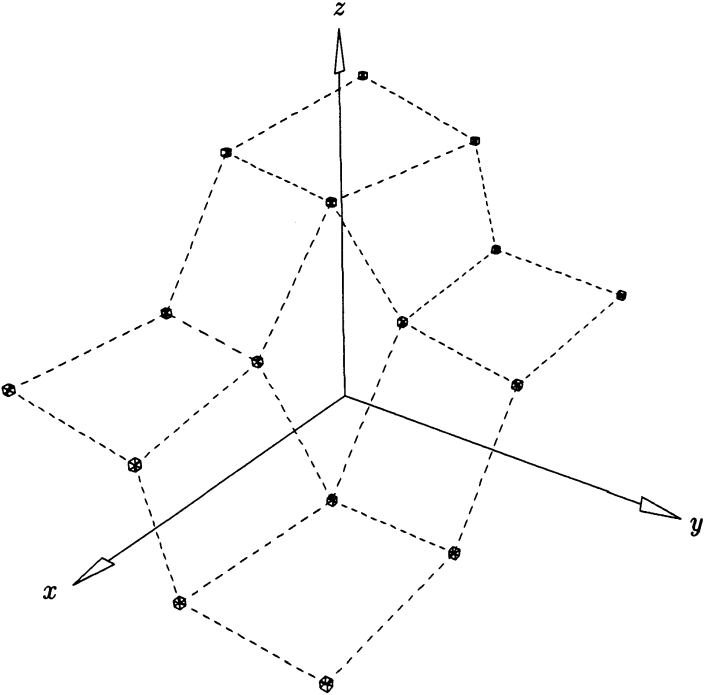
\includegraphics[keepaspectratio, width=5cm]{gambar/Interpolasi/pic11.png}
		\caption{\textit{Data set}}
		\label{gambar:datasetlocal}
	\end{subfigure}%
	\begin{subfigure}{.5\textwidth}
		\centering
		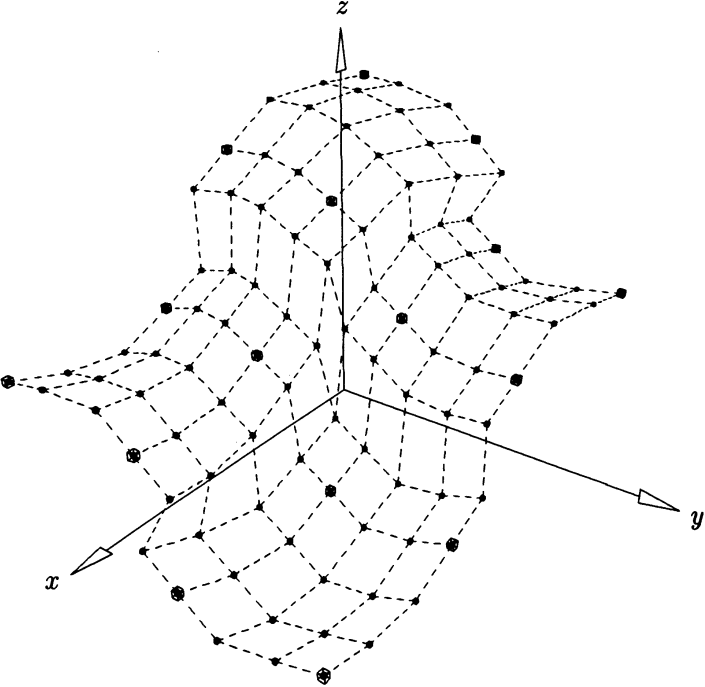
\includegraphics[keepaspectratio, width=5cm]{gambar/Interpolasi/pic12.png}
		\caption{jaring Bézier dari interpolant}
		\label{gambar:beziernet}
	\end{subfigure} \\
	\begin{subfigure}{.5\textwidth}
		\centering
		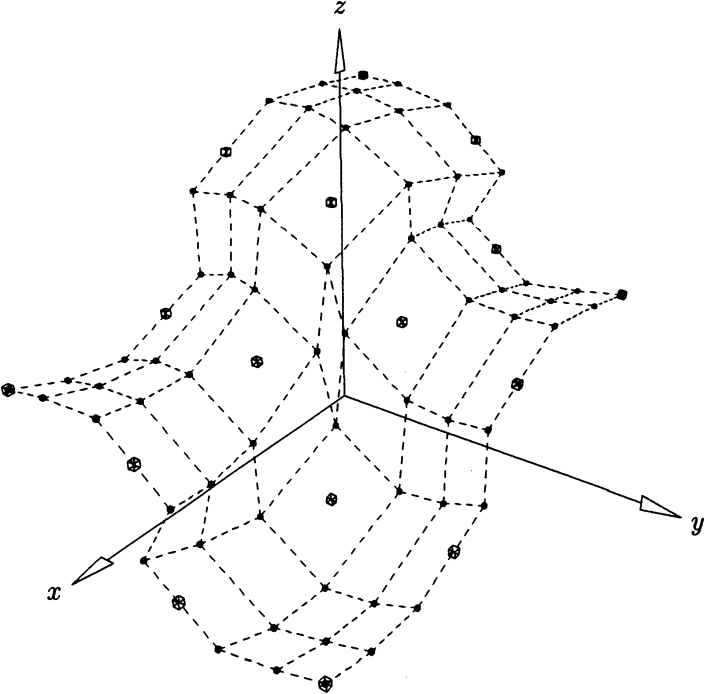
\includegraphics[keepaspectratio, width=5cm]{gambar/Interpolasi/pic13.png}
		\caption{jaring \textit{B-spline} (lingkaran besar menandai 
		titik data, dan lingkaran kecil menandai titik 
		kontrol \textit{B-spline})}
		\label{gambar:beziernetdetail}
	\end{subfigure}%
	\begin{subfigure}{.5\textwidth}
		\centering
		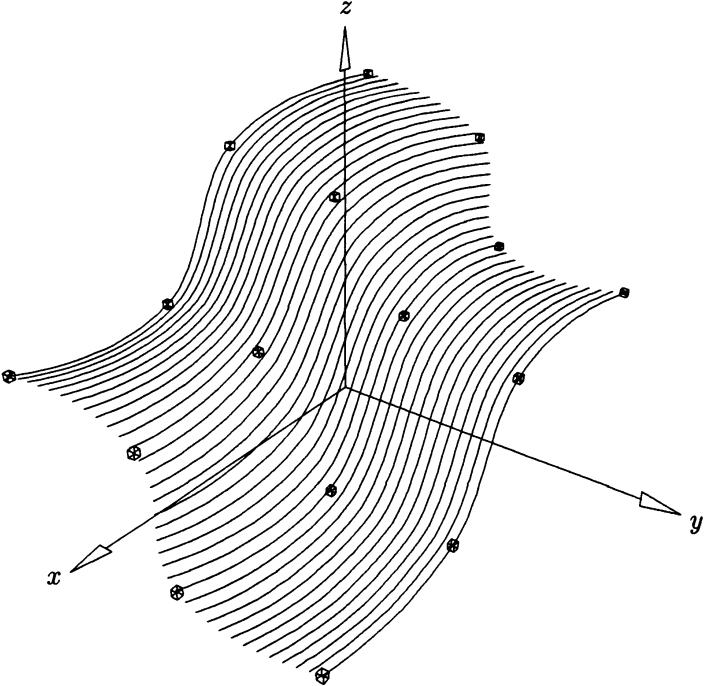
\includegraphics[keepaspectratio, width=5cm]{gambar/Interpolasi/pic14.png}
		\caption{interpolsi permukaan.}
		\label{gambar:surfaceinterpolant}
	\end{subfigure}
	\caption{$C^{(1,1)}$ Interpolasi permukaan bikubik lokal}
\end{figure}

Tambalan bikubik Bézier memiliki 16 titik kontrol. 
12 titik kontrol perbatasan diperoleh dengan awalnya 
melakukan looping melalui $m + 1$ baris dan $n + 1$ 
kolom data dan menggunakan skema interpolasi kurva 
kubik. Skemanya sedikit berbeda dengan detail 
sebelumnya, karena sudah mempunyai parameternya 
{$(\bar{u}_k, \bar{v}_k)$}. Perhatikan bahwa ini harus 
dikomputasi terlebih dahulu, karena semua baris (kolom) 
harus memiliki parameterisasi yang sama pada permukaan 
produk tensor. Dengan demikian, masih dapat 
memaksakan kontinuitas $C^1$ pada titik akhir segmen, 
namun tidak dapat dipaksakan kecepatan yang 
sama pada titik tengah segmen kurva Bézier. Lebih 
spesifik lagi, misalkan $l = l_0$ tetap, dan perhatikan 
kurva kubik yang menginterpolasi titik-titik $\textbf{Q}_{0,l_0} 
, ..., \textbf{Q}_{n,l_0}$. Misalkan $r_{l_0}$ menyatakan 
jumlah chord length pada baris ke-$l_0$. Pada setiap titik, 
$\textbf{Q}_{k,l_0}$, hitung $\textbf{T}_{k,l_0}^u$, 
(satuan tangen pada arah $u$) seperti sebelumnya 
(Persamaan (\ref{rumus:tangenlokal}), (\ref{rumus:alfalokal2}), 
dan (\ref{rumus:turunanlimatitik})). Kemudian titik-titik 
\textit{interior} Bézier pada baris ini dikomputasi dengan
\begin{equation}
	\textbf{P}_{1,0}^{k,l_0}=\textbf{Q}_{k,l_0}+a\textbf{T}_{k,l_0}^u \quad
	\textbf{P}_{2,0}^{k,l_0}=\textbf{Q}_{k+1,l_0}+a\textbf{T}_{k+1,l_0}^u 	
\end{equation}
dimana \[a=\frac{r_{l_0}(\bar{u}_{k+1}-\bar{u}_k)}{3}=
\frac{r_{l_0}\Delta\bar{u}_{k+1}}{3}\]
Kurva yang dihasilkan adalah kontinu $C^1$, dengan 
besaran turunan sama dengan $r_{l_0}$ pada semua 
$\textbf{Q}_{k,l_0}$. Teknik yang sama diterapkan 
pada $n + 1$ kolom data.

ini kembali pada menghitung \textit{interior} empat 
titik kontrol dari setiap patch Bézier. Hal ini memerlukan 
estimasi untuk turunan parsial campuran, $\textbf{D}_{k,l}^{uv}$, 
pada setiap $\textbf{Q}_{k,l}$. diperoleh 
rumus untuk $\textbf{Q}_{k,l}$ berdasarkan metode 
tiga titik Bessel (Persamaan (\ref{rumus:turunanlokal}), 
(\ref{rumus:alfalokal}), dan (\ref{rumus:turunantigatitik})). 
Misalkan $r_l$ dan $s_k$ menyatakan jumlah \textit{chord length} 
pada baris ke-$l$ (kolom ke-$k$). Kemudian
\begin{equation}
	\textbf{D}_{k,l}^u = r_l \textbf{T}_{k,l}^u \quad
	\textbf{D}_{k,l}^v = s_k \textbf{T}_{k,l}^v 
\end{equation}
lalu bentuk \[\textbf{d}_{k,l}^{vu} = 
(1-\alpha_k)\frac{\textbf{D}_{k,l}^v - \textbf{D}_{k-1,l}^v}
{\Delta\bar{u}_k} + \alpha_k \frac{\textbf{D}_{k+1,l}^v - 
\textbf{D}_{k,l}^v}{\Delta\bar{u}_{k+1}} \]
dan \[\textbf{d}_{k,l}^{uv} = 
(1-\beta_l)\frac{\textbf{D}_{k,l}^u - \textbf{D}_{k,l-1}^u}
{\Delta\bar{v}_l} + \beta_l \frac{\textbf{D}_{k,l+1}^u - 
\textbf{D}_{k,l}^u}{\Delta\bar{v}_{l+1}} \]
dengan \[\alpha_k = \frac{\Delta\bar{u}_k}
{\Delta\bar{u}_k + \Delta\bar{u}_{k+1}} \quad
\beta_l = \frac{\Delta\bar{v}_l}
{\Delta\bar{v}_l + \Delta\bar{v}_{l+1}}\]
menjadi
\begin{equation}
	\textbf{D}_{k,l}^{uv} = \frac{\alpha_k \textbf{d}_{k,l}^{uv} +
	\beta_l \textbf{d}_{k,l}^{vu}}{\alpha_k + \beta_l}
	\label{rumus:turunanterakhir}
\end{equation}

Rumus akhir yang sesuai (Persamaan (\ref{rumus:turunantigatitik})) 
harus digunakan pada pembatasnya. Empat \textit{interior} 
titik kontrol pada tambalan ke-($k, l$) sekarang 
dihitung menggunakan Persamaan. (\ref{rumus:turunanterakhir})
\begin{equation}
	\begin{split}
		\textbf{P}_{1,1}^{k,l} &= \gamma\textbf{D}_{k,l}^{uv} + 
		\textbf{P}_{0,1}^{k,l} + \textbf{P}_{1,0}^{k,l} -
		\textbf{P}_{0,0}^{k,l} \\%1
		\textbf{P}_{2,1}^{k,l} &= -\gamma\textbf{D}_{k+1,l}^{uv} + 
		\textbf{P}_{3,1}^{k,l} - \textbf{P}_{3,0}^{k,l} + 
		\textbf{P}_{2,0}^{k,l} \\%2
		\textbf{P}_{1,2}^{k,l} &= -\gamma\textbf{D}_{k,l+1}^{uv} + 
		\textbf{P}_{1,3}^{k,l} - \textbf{P}_{0,3}^{k,l} + 
		\textbf{P}_{0,2}^{k,l} \\%3
		\textbf{P}_{2,2}^{k,l} &= \gamma\textbf{D}_{k+1,l+1}^{uv} + 
		\textbf{P}_{2,3}^{k,l} + \textbf{P}_{3,2}^{k,l} -
		\textbf{P}_{3,3}^{k,l} %4
	\end{split}
\end{equation}
dimana \[\gamma = \frac{\Delta\bar{u}_k+1
\Delta\bar{v}_l+1}{9}\]

% Baris ini digunakan untuk membantu dalam melakukan sitasi
% Karena diapit dengan comment, maka baris ini akan diabaikan
% oleh compiler LaTeX.
\begin{comment}
\bibliography{daftar-pustaka}
\end{comment}